% Generated by experiments/paper_figures.py. Do not edit.
\definecolor{ttgray}{HTML}{9A9893}\definecolor{ttblue}{HTML}{2A78D6}\definecolor{ttorange}{HTML}{EB6834}\definecolor{ttaqua}{HTML}{1BAF7A}\definecolor{ttgrid}{HTML}{DDDCD8}\definecolor{ttmuted}{HTML}{52514E}
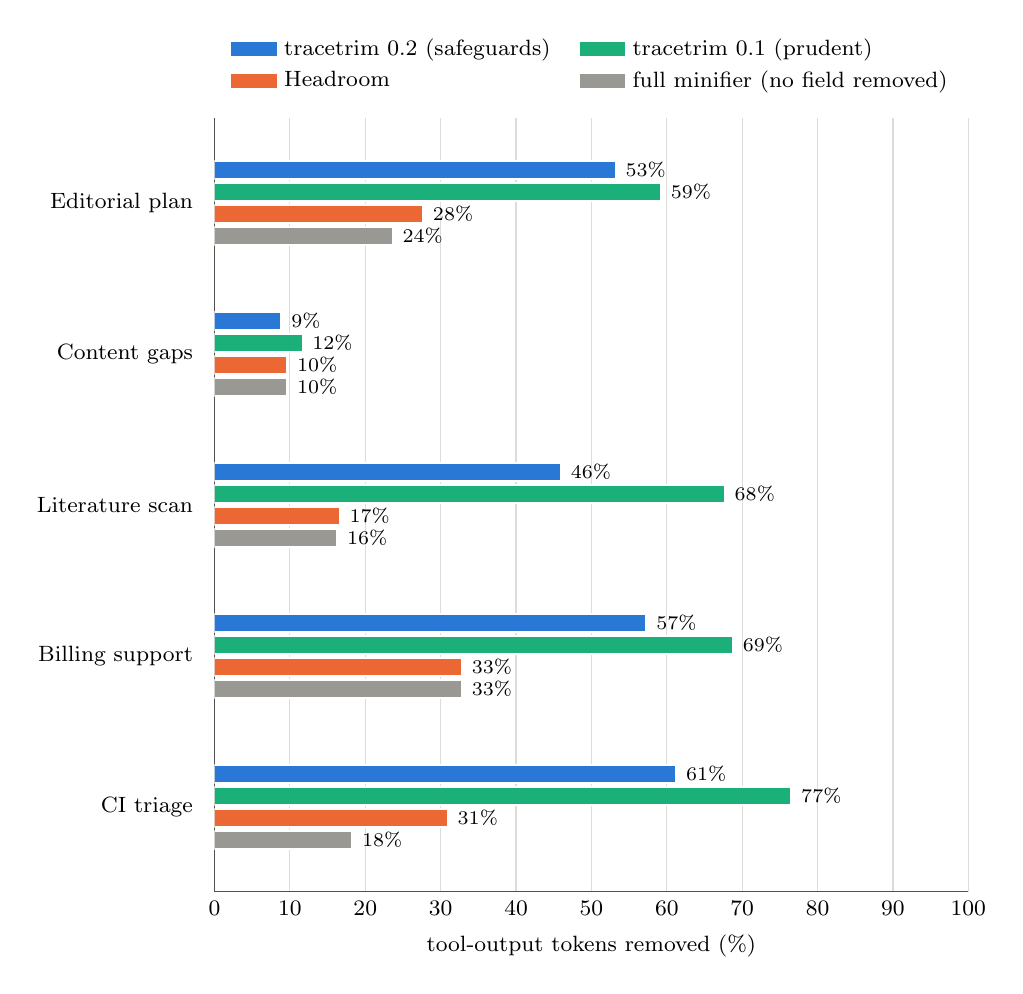
\begin{tikzpicture}
\begin{axis}[axis x line*=bottom, axis y line*=left, axis line style={draw=ttmuted}, tick style={draw=none}, major grid style={draw=ttgrid}, tick label style={font=\footnotesize}, label style={font=\footnotesize}, legend style={font=\footnotesize, draw=none, fill=none}, legend cell align=left, width=0.92\linewidth, height=11.4cm, xbar=1.5pt, xmin=0, xmax=100, area legend, xmajorgrids, xlabel={tool-output tokens removed (\%)}, symbolic y coords={{Editorial plan},{Content gaps},{Literature scan},{Billing support},{CI triage}}, ytick=data, y dir=reverse, enlarge y limits=0.14, legend style={at={(0.5,1.02)}, anchor=south, legend columns=2, /tikz/every even column/.append style={column sep=8pt}}, reverse legend]
\addplot[xbar, bar width=6.5pt, fill=ttgray, draw=white, line width=0.6pt, nodes near coords={\pgfmathprintnumber[fixed,precision=0]{\pgfplotspointmeta}\%}, nodes near coords style={font=\scriptsize, text=black, anchor=west}] coordinates {(23.6279,{Editorial plan}) (9.6340,{Content gaps}) (16.2676,{Literature scan}) (32.7978,{Billing support}) (18.2565,{CI triage})};
\addlegendentry{full minifier (no field removed)}
\addplot[xbar, bar width=6.5pt, fill=ttorange, draw=white, line width=0.6pt, nodes near coords={\pgfmathprintnumber[fixed,precision=0]{\pgfplotspointmeta}\%}, nodes near coords style={font=\scriptsize, text=black, anchor=west}] coordinates {(27.6527,{Editorial plan}) (9.6340,{Content gaps}) (16.5908,{Literature scan}) (32.7978,{Billing support}) (30.9312,{CI triage})};
\addlegendentry{Headroom}
\addplot[xbar, bar width=6.5pt, fill=ttaqua, draw=white, line width=0.6pt, nodes near coords={\pgfmathprintnumber[fixed,precision=0]{\pgfplotspointmeta}\%}, nodes near coords style={font=\scriptsize, text=black, anchor=west}] coordinates {(59.2083,{Editorial plan}) (11.6582,{Content gaps}) (67.6744,{Literature scan}) (68.7614,{Billing support}) (76.5005,{CI triage})};
\addlegendentry{tracetrim 0.1 (prudent)}
\addplot[xbar, bar width=6.5pt, fill=ttblue, draw=white, line width=0.6pt, nodes near coords={\pgfmathprintnumber[fixed,precision=0]{\pgfplotspointmeta}\%}, nodes near coords style={font=\scriptsize, text=black, anchor=west}] coordinates {(53.1967,{Editorial plan}) (8.8536,{Content gaps}) (45.9463,{Literature scan}) (57.2795,{Billing support}) (61.2196,{CI triage})};
\addlegendentry{tracetrim 0.2 (safeguards)}
\end{axis}
\end{tikzpicture}
